\documentclass{beamer}

% Used packages
\usepackage{graphicx}
\usepackage{hyperref}
\usepackage{algorithm}
\usepackage{array}
%\usepackage{algpseudocode}
    \renewcommand{\arraystretch}{1.8}
% The title
\title[Code Mobility]{Code Mobility}

% The date
\date{\today}

% The author
\author[Jakovljevi\'c,Selyunin,Pelesi\'c]{
 \Large{Konstantin Selyunin}\\
  \small{\texttt{e1228206@student.tuwien.ac.at}}\\
 \Large{Miljenko Jakovljevi\'c}\\
  \small{\texttt{e1228206@student.tuwien.ac.at}}\\
  \Large{Igor Pelesi\'c}\\
  \small{\texttt{e0006828@student.tuwien.ac.at}}\\
}

% Use Warsaw theme
\usetheme{Warsaw}

% New commands
\newcommand{\mc}[1]{$\mathcal{#1}$}

\theoremstyle{definition} \newtheorem{mdefinition}{Definition}
\theoremstyle{plain} \newtheorem{mtheorem}{Theorem}
\theoremstyle{plain} \newtheorem{mcorollary}{Corollary}
\theoremstyle{plain} \newtheorem{mfact}{Fact}

% Begin of document
\begin{document}

\begin{frame}
	\titlepage
\end{frame}

\begin{frame}
	\frametitle{Outline}
	\tableofcontents
\end{frame}

\section{Introduction}
\subsection{Motivation}
\begin{frame}[fragile]
	\frametitle{Motivation}
% 	\framesubtitle{}
	\begin{itemize}
		\item Design code mobility system on ESE Board
		\item Practical experience
		\item Project management skills
	\end{itemize}
\end{frame}

\subsection{Code mobility overview}
\begin{frame}
	\frametitle{Code mobility overview}
 		\framesubtitle{Concept of code mobility}
	\begin{block}{Concept of code mobility}
		\begin{description}
			\item	Mobile agents
			\item	Meta-level knowledge
			\item   Layered architecture
			\item	{\it Strong} and {\it weak} code mobility
		\end{description}
	\end{block}

	\begin{block}{Advantages of code mobility}
		\begin{description}
			\item	Move code close to resources 
			\item	Enable client customization of remote resources
			\item	Performance gains
		\end{description}
	\end{block}	

\end{frame}

\subsection{Level of abstraction}
\begin{frame}
\frametitle{Level of abstraction}
\begin{centering}
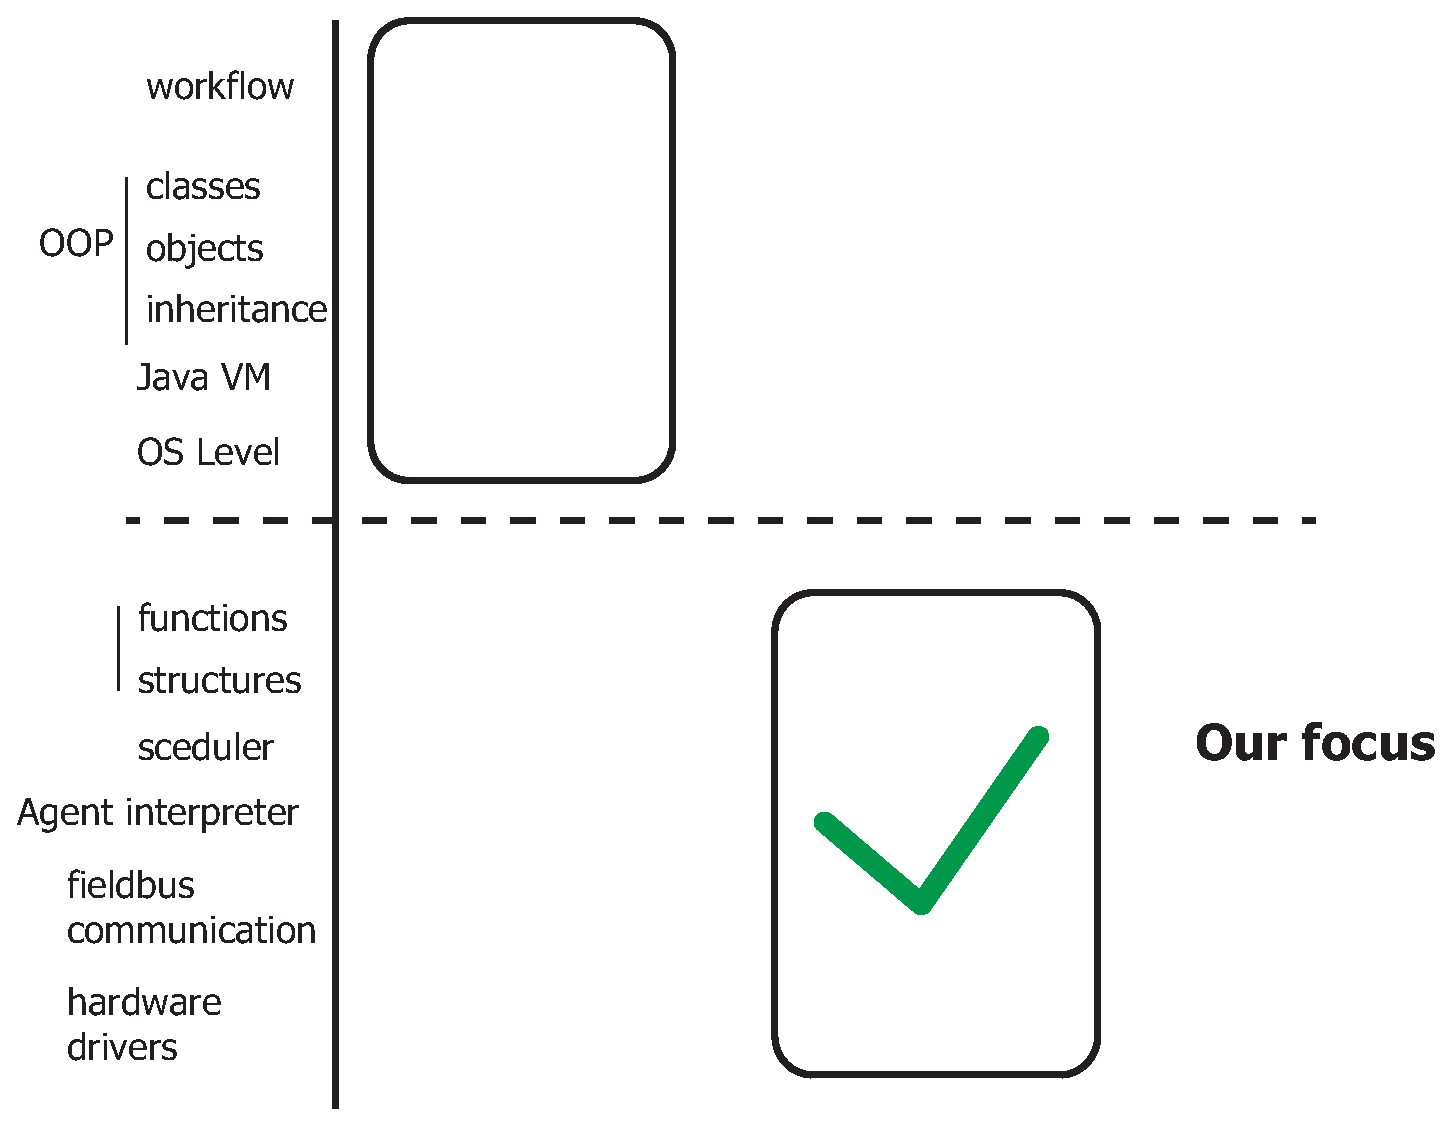
\includegraphics[width=3in]{img/abstraction-3}
\end{centering}
\end{frame}

\subsection{Design challenges for the project}
\begin{frame}
\frametitle{Design challenges for the project}
\begin{tabular}{ll}
Processing gap & \\

Performance & \\

Memory management & \\

Communication design & \\
\end{tabular}

\end{frame}

\subsection{Requirements}
\begin{frame}
	\frametitle{Requirements}
% 	\framesubtitle{}
%To develop a solution that allow to trasfer code from one platform to another

\begin{itemize}
	\item Agents:
	\begin{itemize}
		\item simple language 
		\item support mobility and message exchange
	\end{itemize} 
	\item Platform:
	\begin{itemize}
		\item execute agents concurrently
		\item provide hardware services to agents
	\end{itemize}	
	\item Communication:
	\begin{itemize}
		\item transfer agents \& state {\it strong mobility}
		\item transfer messages between platforms
		\item cross board communication via Zigbee
	\end{itemize}
\end{itemize}
\end{frame}

\section{System architecture}
\subsection{General overview}
\begin{frame}
	\frametitle{General overview}
% 	\framesubtitle{}
	%Three level archtecture
\begin{columns}[c]
\column{1.5in}
	3 layered architecture:
		\begin{itemize}
		\item Agent level
		\item Platform level
		\item communication \& drivers
		\end{itemize}
\column{2in}
\includegraphics<1>[height=2in]{img/overview_1}
\includegraphics<2>[height=2in]{img/overview_2}

\end{columns}
\end{frame}

\subsection{Agents}

\begin{frame}
	\frametitle{Agent language that support:}
	\begin{itemize}
	\item Arithmetical operations, branching and looping
	\item Message exchange
	\item Replication and code mobility
	\end{itemize}
% 	\framesubtitle{}

\end{frame}

\begin{frame}
	\frametitle{Agents}
\includegraphics<1>[width=4in]{img/agent-1}
\includegraphics<2>[width=4in]{img/agent-2}
\includegraphics<3>[width=4in]{img/agent-3}
\includegraphics<4>[width=4in]{img/agent-4}	
% 	\framesubtitle{}

\end{frame}

\subsection{Platform}
\begin{frame}
	\frametitle{Platform}
% 	\framesubtitle{}
\begin{center}
\includegraphics<1>[scale=0.29]{img/plat1} 
\end{center}



\end{frame}

\subsubsection{Scheduler}
\begin{frame}
	\frametitle{Scheduler}
% 	\framesubtitle{}

\begin{center}
\includegraphics<1>[scale=0.27]{img/plat2} 
\end{center}

\end{frame}


\subsubsection{Execution Layer}
\begin{frame}
	\frametitle{Execution Layer}
% 	\framesubtitle{}
\begin{center}
\includegraphics<1>[scale=0.29]{img/plat3} 
\end{center}


\end{frame}


\subsection{Communication}
\begin{frame}
	\frametitle{Communication}
% 	\framesubtitle{}

\end{frame}

\section{Project management}
\begin{frame}
	\frametitle{Milestones}
%	\begin{itemize}
%	\item Phase 1. Product outline and information gathering 
%	\item Phase 2. Application requirements and specification
%	\item Phase 3. Implementation
%	\item Phase 4. Validation and analysis
%	\end{itemize}

\begin{tabular}{ll}


\includegraphics[]{img/milestone} & Phase 1. Product outline and information gathering\\

\includegraphics[]{img/milestone} & Phase 2. Application requirements and specification\\

\includegraphics[]{img/milestone} & Phase 3. Implementation\\

\includegraphics[]{img/milestone} & Phase 4. Validation and analysis\\
\end{tabular}

% 	\framesubtitle{}

\end{frame}

\begin{frame}
	\frametitle{Workpackages}
% 	\framesubtitle{}
\end{frame}


\begin{frame}
	\frametitle{Gantt diagram}

\begin{center}
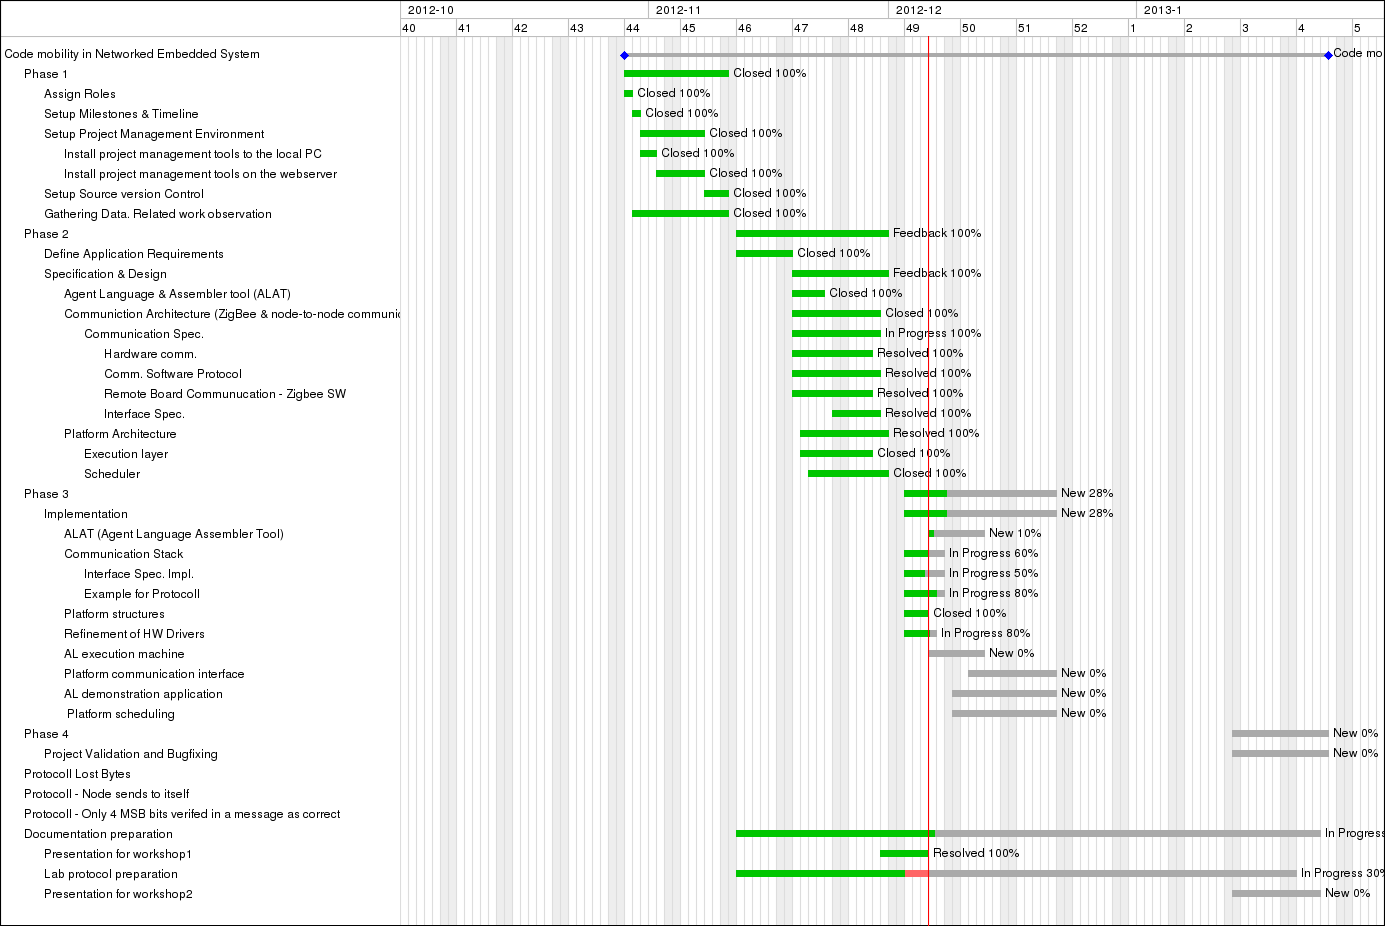
\includegraphics[height=2.7in]{img/gantt}

\end{center}
\end{frame}

\section{Tools}

\begin{frame}
	\frametitle{Tools}

\begin{tabular}{lcl}

Version control & 
\includegraphics[width=0.07\textwidth]{img/gitlogo} & git\\
Documentation \& code repository & 
\includegraphics[width=0.07\textwidth]{img/github-logo} & github\\
File sharing & 
\includegraphics[width=0.1\textwidth]{img/aws-logo} & amazon s3\\
Project management & 
\includegraphics[width=0.07\textwidth]{img/redmine-logo} & redmine\\
Code generation & 
\includegraphics[width=0.07\textwidth]{img/scade-logo} & SCADE\\
Editors & 
\includegraphics[width=0.07\textwidth]{img/emacs-logo} & Emacs\\
        & & gedit\\

\end{tabular}

\end{frame}

% End of document
\end{document}
